\chapter{مقدمه}
با پیشرفت شبکه‌های تلفن همراه، پیچیدگی این شبکه‌ها نیز بیش‌تر شده‌است و این مدیریت این شبکه‌ها را سخت‌تر از گذشته کرده ‌است و این نیاز را ایجاد کرده ‌است که مدیریت و بهینه‌کردن پیوسته‌ی این شبکه‌ها در محیط عملیاتی به صورت خودکار انجام شود. 

همان طور که در 
\ref{fig:ran}
می‌بینیم، شبکه‌های تلفن‌همراه از ۳ بخش اصلی تشکیل شده اند و ناحیه‌ی دسترسی رادیویی است که تلفن همراه یا همان کاربر را به هسته‌ی شبکه متصل می‌کند.
\begin{figure}[H]
	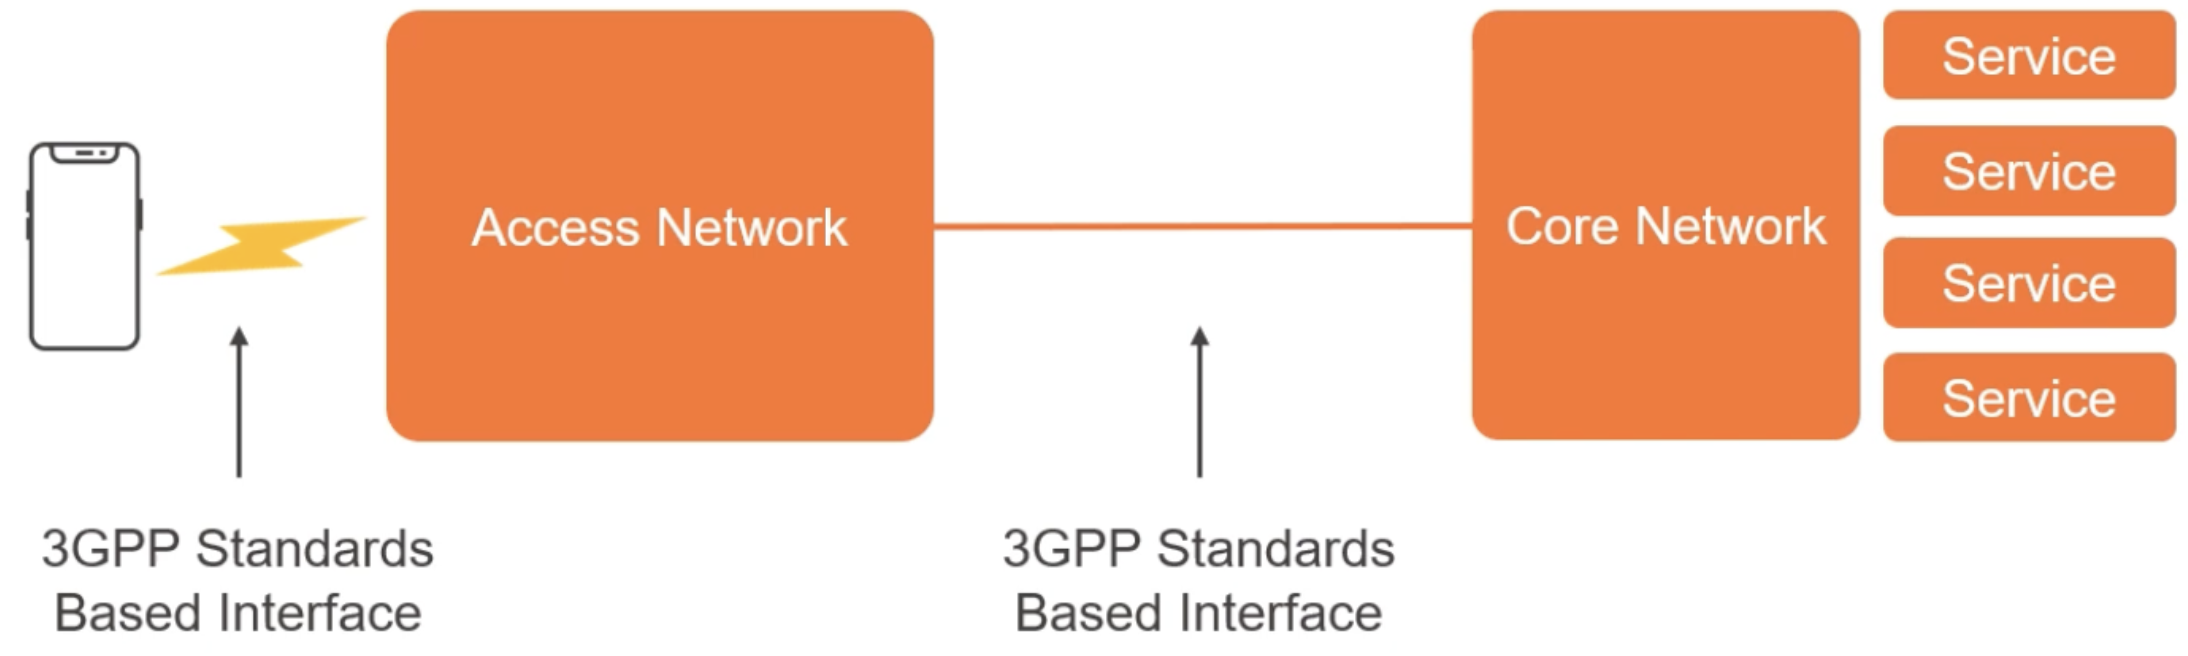
\includegraphics[width=0.85\columnwidth]{Picture/ran.png}
	\centering
	\caption{معماری کلی شبکه‌های تلفن همراه}
	\label{fig:ran}
\end{figure}

ناحیه دسترسی رادیویی تا مدت‌ها به صورت یک قسمت یک‌پارچه بوده و اطلاعاتی از کارهایی که درون آن انجام می‌شده به قسمت‌های دیگر برای بهینه‌سازی آن داده نمی‌شده و بسیار وابستگی به فروشنده
\LTRfootnote{vendor}
سازنده‌ی آن داشته است.
\lr{3GPP}
به عنوان سازمان استاندارسازی شبکه‌های تلفن همراه در نسخه‌های جدیدی که از نسل ۵ شبکه‌های تلفن همراه منتشر کرده‌است، ناحیه دسترسی رادیویی را جداسازی کرده و آن را به ۳ قسمت تفکیک کرده‌است. در 
\ref{fig:3gpp-ran}
این ۳ قسمت قابل مشاهده‌ هستند. با این تفکیک و ایجاد قسمت‌های 
\lr{RU}
\lr{DU}،
و 
\lr{CU}
باید واسط‌های ارتباطی جدیدی برای ارتباط این قسمت‌ها تعریف می‌شد که این موارد نیز در این شکل مشاهده می‌شوند. به عنوان مثال 
\lr{Fronthaul}
واسط بین بخش‌های 
\lr{RU}
و 
\lr{DU}
است.
\begin{figure}[H]
	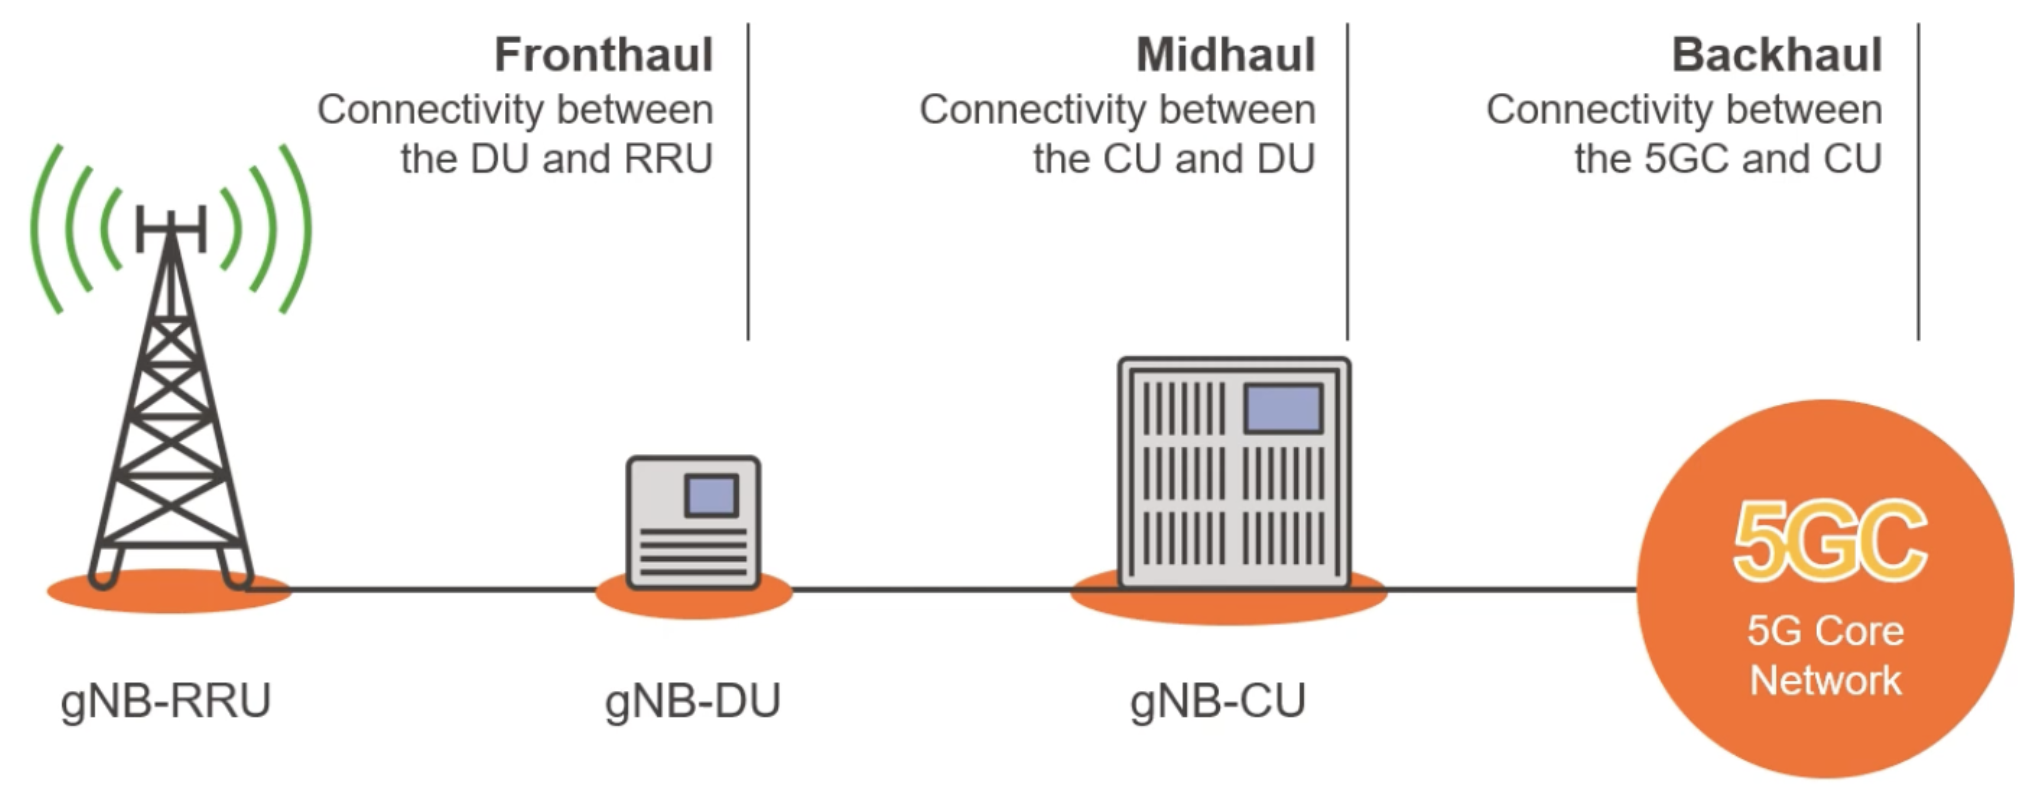
\includegraphics[width=0.85\columnwidth]{Picture/3gpp-ran.png}
	\centering
	\caption{تفکیک ناحیه‌ی رادیویی نسل ۵ توسط
	\lr{3GPP}}
	\label{fig:3gpp-ran}
\end{figure}

اگر عملکرد این قسمت‌های جدید را در پشته‌ی پروتکلی شبکه‌های تلفن همراه هم بررسی کنیم، می‌توانیم وظایف موجود در هر کدام از لایه‌های مختلف را به یکی از این قسمت‌های جدید در ناحیه دسترسی رادیویی واگذار کنیم. در 
\ref{fig:prot-stack}
می‌بینیم که این لایه‌ها می‌توانند به شیوه‌های مختلفی به 
\lr{RU}
\lr{DU}،
و 
\lr{CU}
اختصاص یابند که این مسئله قابل پیکره‌بندی است.

\begin{figure}[H]
	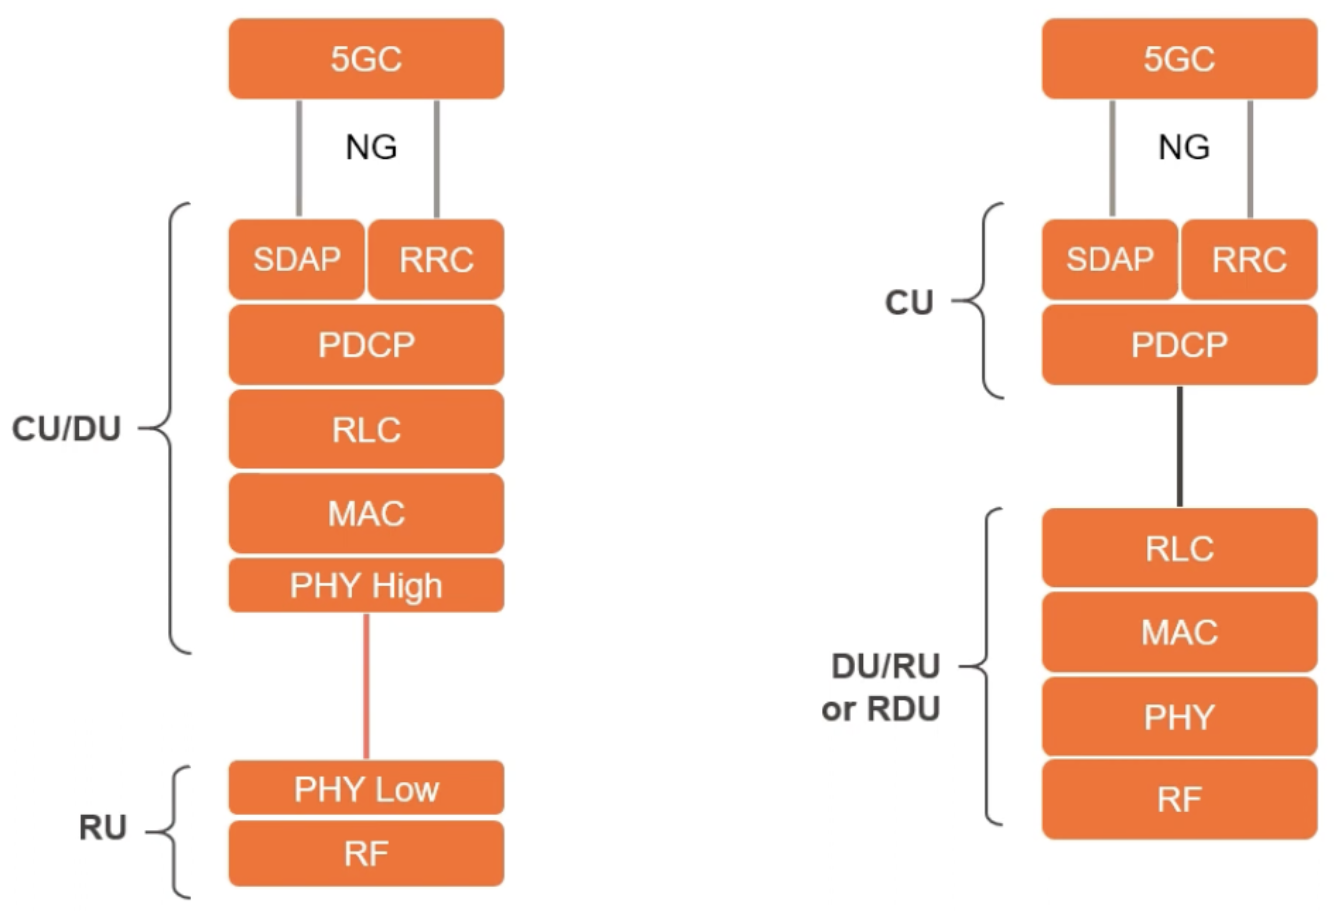
\includegraphics[width=0.85\columnwidth]{Picture/prot-stack.png}
	\centering
	\caption{قسمت‌بندی‌های مختلف لایه‌های شبکه‌}
	\label{fig:prot-stack}
\end{figure}

در ادامه‌ی این راه و برای توسعه‌ی بیش‌تر این رویکرد خارج کردن ناحیه‌ی رادیویی از انحصارطلبی گذشته، سازمانی تحت عنوان
\lr{O-RAN Alliance} 
تشکیل شد که هدف آن تمرکز بر همین ایده و پیش‌برد ایده‌ی ناحیه‌ی دسترسی رادیویی آزادتر و هوشمندتر بود.

\begin{figure}[H]
	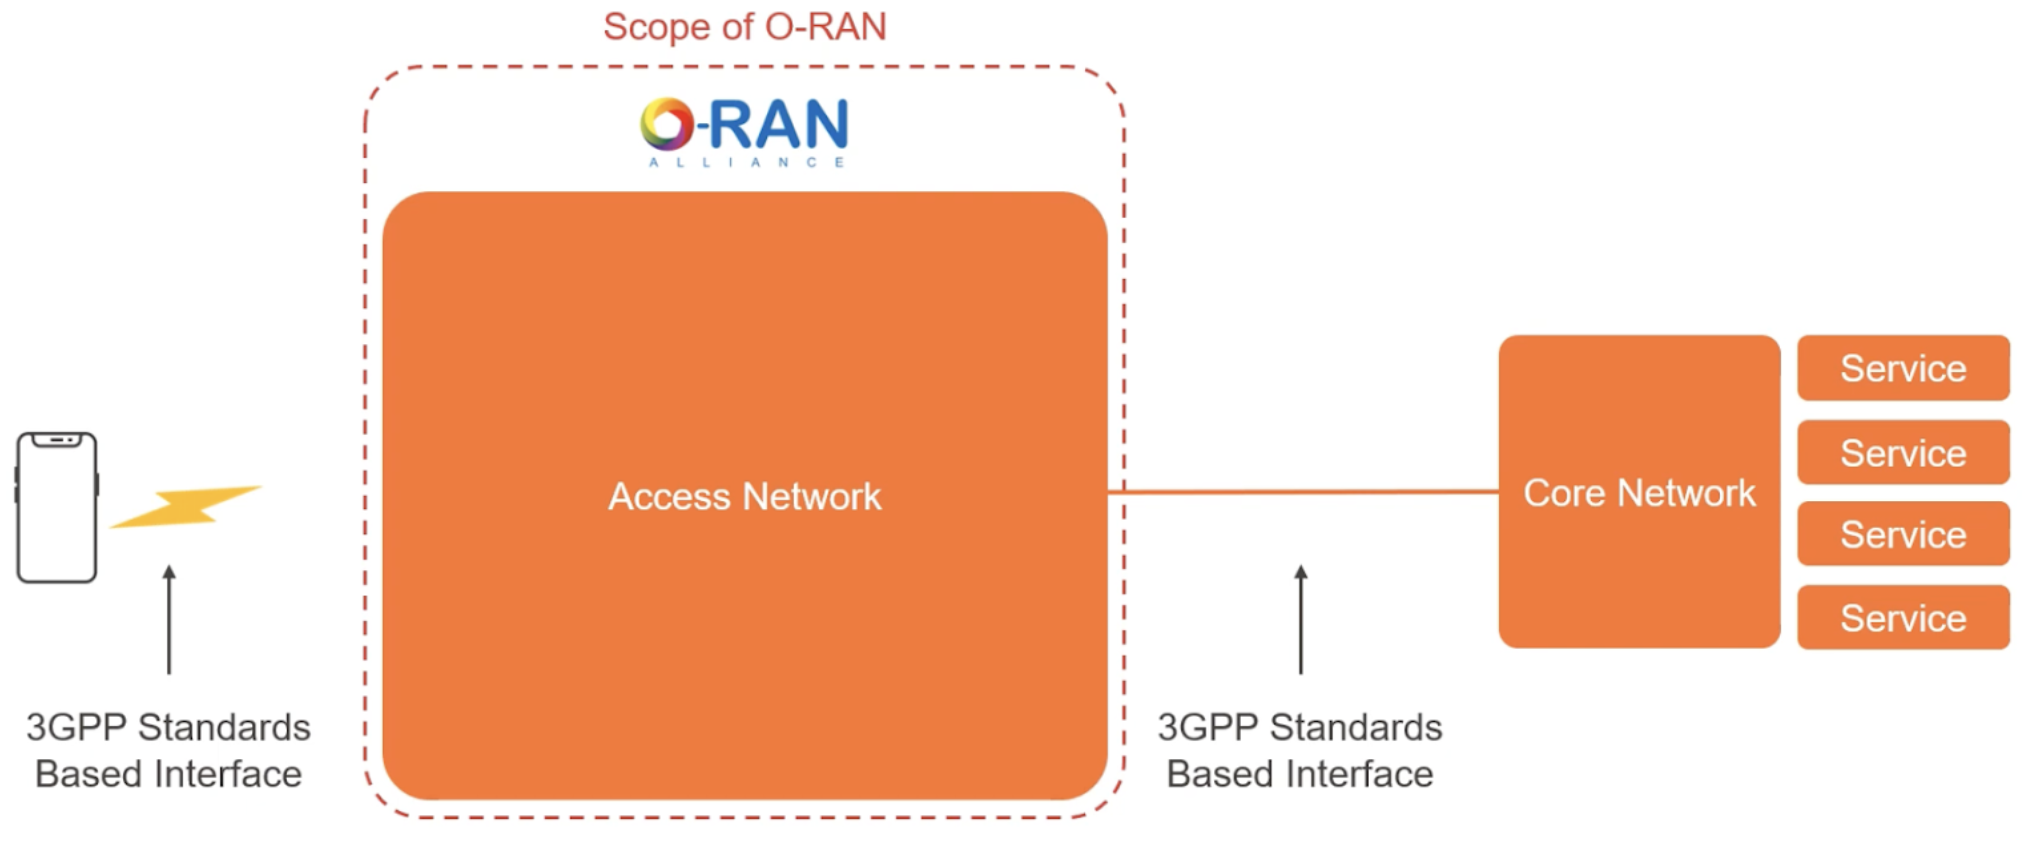
\includegraphics[width=0.85\columnwidth]{Picture/alliance.png}
	\centering
	\caption{تمرکز کاری
	\lr{O-RAN Alliance}}
	\label{fig:alliance}
\end{figure}

در فصل‌های بعدی با کمک
\cite{oran2022-tutorial}
و
\cite{parallelwireless_2021}
 معماری کنونی 
\lr{O-RAN} 
که توسط این سازمان استاندارشده را بررسی خواهیم کرد.

\begin{note}
سازمان 
\lr{O-RAN Alliance} 
بر استانداردسازی‌های 
\lr{O-RAN}
تمرکز کرده است و با همکاری
\lr{Linux Foundation}
که یک سازمان متن‌باز است، مجموعه‌ی 
\lr{O-RAN Software Community}
را تشکیل داده‌است که وظیفه‌ی توسعه‌ی مواردی که استاندارد می‌شود را به صورت متن‌باز پیش می‌برند و به صورت پیوسته برای قسمت‌های مختلف این معماری، پیاده‌سازی‌هایی انجام می‌دهند.
\end{note}






